\chapter{Introduction}
\label{chapter:introduction}

The day is September 27, 1908. The first Ford Model T has left the factory and with it the history of the automobile and transportation was forever changed~\cite{Ford, JohnSteeleGordon2007}. The Model T was not the first automobile, neither the first powered wheeled vehicle, but was the first mass-produced car in an assembly line~\cite{JohnSteeleGordon2007, DailyNews2013}. Other vehicles have preceded it, from steam carriages and coaches on the Victorian Era of Steam and electrical cars in 1888~\cite{PaulA.Hughes}, to internal combustion engines with hydrogen, kerosene and crude~\cite{Setright2003}; but none was so influential, memorable and widely adopted. 

The model T and other automobiles at an affordable price proliferated, allowing the middle-wage class to own motorized vehicles~\cite{JohnSteeleGordon2007, DailyNews2013}. The massification of such vehicles, while improving mobility of the middle class on a society at the brink of modern industrialization, started what is now one of the leading causes of mortality in the world: road accidents~\cite{WHO2018}. On the United States of America, such events triggered the foundation of the Automobile Safety League of America in 1930, which enforced the usage of seatbelts and padded dashboards. However, several decades would have to unfold before road safety became a major concern for governments, automobile manufactures, urban planners and \acp{ngo}. 

Despite all the efforts and technological advances, the number of annual global road traffic deaths is rising and it reached 1.35 million in 2018, being the leading cause of death for people aged 5 to 29 years~\cite{WHO2018}. That means that every 23 seconds a road user will die from an accident% (or 5 people since you started reading this introduction)
~\cite{WHOvisualizer}. Actions from multidisciplinary partners are being taken to reduce this growing number, such as road safety awareness campaigns, heavier fines, stricter regulations on road and automobile safety, inspection operations and driver assistance systems~\cite{WHO2018, EUroads}. However, only 40 countries in the world have legislated on road safety and vehicle manufacturing that follows the 7 most important directives on road safety issued by \acf{who}~\cite{WHOvisualizer}. The list of countries with non-conforming legislation includes not only ``developed'' countries from Europe and the United States of America, but also ``sub-developed'' countries in Asia and Africa (see more statistics in Figure~\ref{fig:who-media}).

Backed both by common sense and research, human error is still the leading cause of accidents and injuries on the road~\cite{Bimbraw2015, WHO2018}, causing up to 90\% of the road accidents~\cite{WHO2018}. Distractions, fatigue, bad decisions and reckless behavior are some main reasons for human error. To reduce this grim number, manufacturers and tech companies put their efforts on developing driving systems that can aid drivers making decisions or even systems that make decisions on their own, such as adaptive headlamps and collision avoidance systems, respectively.


\begin{figure}[!ht]
	\centering
	\begin{subfigure}[c]{0.3\textwidth}
		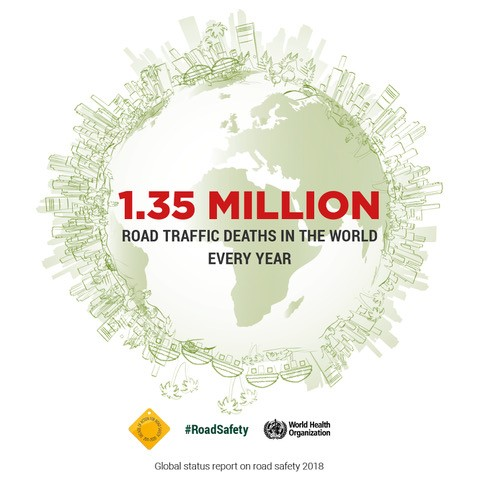
\includegraphics[width=\textwidth]{img/road_safety/1_35-million.jpg}
		%\caption{Picture 1}
		\label{fig:test_image_1}
	\end{subfigure}
	\quad
	\begin{subfigure}[c]{0.3\textwidth}
		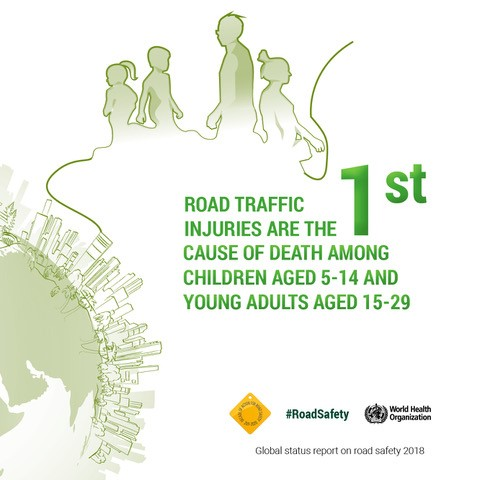
\includegraphics[width=\textwidth]{img/road_safety/1st-cause.jpg}
		%\caption{Picture 1}
		\label{fig:test_image_2}
	\end{subfigure}
	\quad
	\begin{subfigure}[c]{0.3\textwidth}
		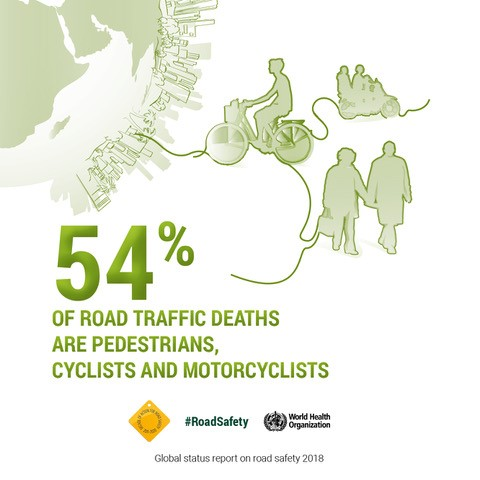
\includegraphics[width=\textwidth]{img/road_safety/54-percent-deaths.jpg}
		%\caption{Picture 1}
		\label{fig:test_image_3}
	\end{subfigure}
	\medskip
	\begin{subfigure}[c]{0.3\textwidth}
		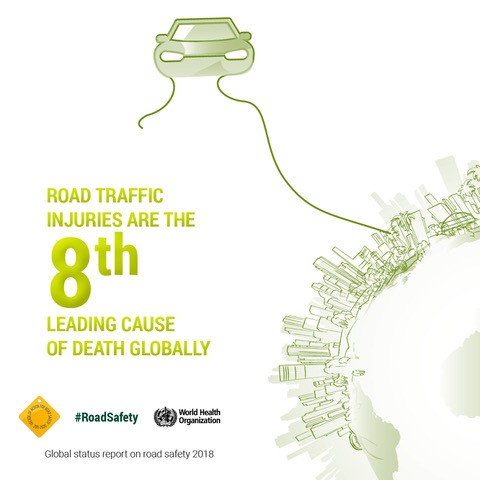
\includegraphics[width=\textwidth]{img/road_safety/8th-leading-cause.jpg}
		%\caption{Picture 1}
		\label{fig:test_image_4}
	\end{subfigure}
	\quad
	\begin{subfigure}[c]{0.3\textwidth}
		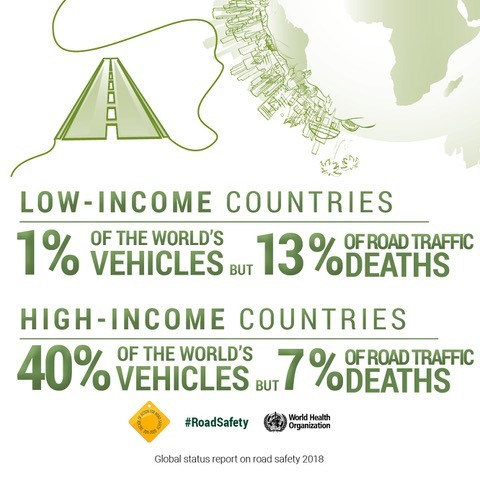
\includegraphics[width=\textwidth]{img/road_safety/Low-income-countries.jpg}
		%\caption{Picture 1}
		\label{fig:test_image_5}
	\end{subfigure}
	\caption[Social media visuals produced by the \acs{who} for raising awareness on road safety.]{Social media visuals produced by the \ac{who} for raising awareness on road safety. The data is available on the Global status report on road safety 2018~\cite{WHO2018} and the graphics material source can be found on \ac{who} website~\cite{WHOsite}.}
	\label{fig:who-media}
\end{figure}

Since the appearance of \ac{adas}, consumers, experts and governments hoped that ``smarter'' cars would result in safer roads. Several studies have been conducted on autonomous driving technology and \ac{adas}~\cite{Fridman2017, ADAS1, Bimbraw2015, Santos2019Atlascar, Santos2019, Santos2017}, which appears as one of the most promising solutions to mitigate road accidents. Research shows that solving or at least reducing the impact of this problem could be ``easy'': remove the human driver from the driving process and replace it with autonomous driving technology. However, the problem of making autonomous driving vehicles is rather complex and has gathered the attention of both technical and non-technical personnel. Newspaper articles, blog posts, podcasts and interviews have been published over the last years, revealing the interest on the topic. \ac{ai}, computer vision and autonomous driving startups have boomed in the last years and tech giants have revealed their plans to conquer this market segment.

The mission of the automobile industry is to improve the way humans move from a place to another, allowing faster, cheaper and more convenient transportation~\cite{Setright2003, DailyNews2013}. % By reshaping society and cities these goals have been attained, yet, some downsides are not solved, such as road safety.
While such a mission has been fulfilled, reshaping society and cities in the process, some of their downsides are yet to be solvable, such as road safety.


\section{Scope and Motivation}
\label{sec:introduction:scope_motivation}
To build an autonomous driving vehicle as the solution to improve road safety, one needs to be capable of perceiving the world surrounding it, both accurately and in real time. The quality
of the data gathered is as crucial as its diversity, which is addressed with the usage of multiple sensors. A multiple sensor approach to autonomous driving allows:

\begin{itemize}
	\item \textbf{Data diversity:} different aspects of the surrounding environment are measured, providing complementary data;
	\item \textbf{Data redundancy:} multiple sensors complement the data gathered by each other, due to measurements of the same physical phenomena with overlapping \ac{fov};
	\item \textbf{Data robustness:} since multiple sensors gather information about the vehicle surroundings in different formats, individual sensor weakness and limitations are circumvented, creating a more realistic and accurate model, even in scenarios where one sensor cannot operate properly or reliably.
\end{itemize}

Autonomous driving vehicles are equipped with a wide range of sensors and systems, from parking sensors, crash detection, traffic signal detection, adaptive headlights, \ac{abs}, adaptive cruise control, among others. Regarding the perception of the environment surrounding the car, the most used sensors are detailed below, with their common position and \ac{fov} being detailed in Figure~\ref{fig:introduction:homer-setup}.

\begin{itemize}
	\item \textbf{Camera:} Most accurate sensor to represent objects, given good visibility conditions. Enables a good semantic view of the world, allowing the car to differentiate objects and understand their actions.  
	\item \textbf{\ac{radar}:} capable of long range object detection, \acp{radar} uses radio waves to detect obstacle distance and velocity. It has a good performance on adverse weather conditions but lacks angular resolution to enable the distinction between different objects (cars, trucks, persons, etc.)
	\item \textbf{\ac{lidar}:} medium range laser sensor that provides an accurate, but sparse, tridimensional view of the world.
	\item \textbf{\ac{sonar}:} small range sensor that uses sound waves to detect with precision obstacles nearby. Commonly used on to allow automatic parking. 
\end{itemize}

\begin{figure}
	\centering
	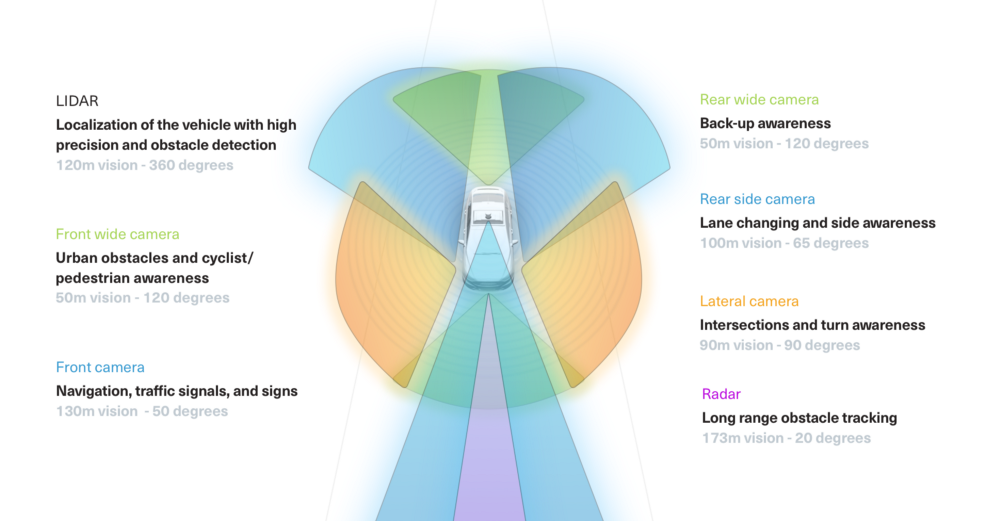
\includegraphics[width=0.8\textwidth]{img/sensor_fusion/homer_setup.png}
	\caption[Example of a multiple sensor setup on an autonomous car.]{Example of a self-driving taxi (Homer) multiple sensor setup and their relative positioning. Source: Voyager~\cite{Cameron}.}
	\label{fig:introduction:homer-setup}
\end{figure}

Since \ac{darpa} Grand Challenge on the Mojave Desert, in 2004 and 2007, modern automotive \ac{lidar} has become one of the leading technologies for autonomous driving cars~\cite{Bezemek2017}. Velodyne reinvented the sensor that is now considered by many automotive companies, tech enthusiasts and experts as the crucial sensor for the fully autonomous driving cars (level 5 automation), due to its precision when creating a tridimensional  model of the surrounding environment. Despite \ac{lidar} technology providing data about the environment that is not attainable with other methods, there is no consensus on the necessity of using \ac{lidar} for autonomous driving. For instance, while some authors believe \ac{lidar} to be indispensable~\cite{Bimbraw2015, Hecht2018, Sullivan2016}, Tesla is building an autonomous driving solution without \acp{lidar}, relying solely on \ac{radar} and cameras (for more information see~\cite{Bimbraw2015, Hecht2018}).


\ac{lidar} sensors map their surroundings because of their capability to precisely measuring depth, with a few centimeters of error, over distances that can range until \SI{100}{\meter}~\cite{VLP16, Sullivan2016} or even \SI{300}{\meter} in certain conditions. This sensor is being employed as the solution to help cars understand the world around them, but there is a caveat that is not being addressed nor deeply considered by the scientific community: \acp{lidar} may inadvertently produce interference.

Since \ac{lidar} is an active sensor, it sends laser pulses (tenths to a few thousand of pulses per second) to the scene. Laser's divergence and the detector's \ac{fov} are small, but what happens when a hundred or thousands cars with \acp{lidar} ``flood'' the streets? Do they interfere mutually, i.e., the laser emitted by a \ac{lidar} on a car ``A'' interferes with the detector of the \ac{lidar} of a car ``B''? And if so, how do they interfere and what are the consequences? 

In a society where the scientific community and automotive manufacturers are concerned about deploying autonomous driving technologies and cars to the streets as soon as possible, and governments lack scientific expertise to legislate on the topic, this research work focuses on understanding what happens if multiple \acp{lidar} interact.

Before autonomous driving cars can replace the human driver and therefore reduce the growing
tendency for road accidents and deaths, we need to understand if the sensors we are using for the vehicles to perceive their surroundings with better accuracy than us are scalable to a scenario when the majority (or even totality) of cars are autonomous. Failing to do so, will not only delay the exciting advent of autonomous driving technology, but also undermine one of the solutions to tackle the ever-growing problem that started such endeavour in the first place: reducing the amount of deaths on the road.

This Master's thesis intends to cast a light on this topic and provide new information about multiple \ac{lidar} interference by simply providing an answer to the question: \textit{What happens if two \acp{lidar} that coexist in the same space are switched on simultaneously?} 


\section{Objectives}
\label{sec:introduction:objectives}
This Master's thesis main objective is to study the behaviour and impact of interference between \acp{lidar}. This study also aims to describe the impact of interference in objects of interest on the \ac{lidar} \ac{fov}. Those objects' position will be estimated by an algorithm to be developed, based on the results of object detection on image.

To do this, and before making any conclusions on \ac{lidar} interference, we must attain several intermediate objectives:
\begin{enumerate}
	\item Implement an algorithm for performing extrinsic calibration between the camera and the \ac{lidar} of the experimental setup;
	\item Merge the information obtained with the camera and the \ac{lidar} to construct a more realistic scenario of the environment;
	\item Detect objects of interest in camera images and estimate their position on the	\ac{lidar} point cloud;
	\item Devise experiments with different metrics being varied and create a rich data set for assessing \ac{lidar} interference.
\end{enumerate}

Fulfilling objective \#1 indicates that we are able to exchange information between different sensors, by converting data between the sensors' coordinate frames, crucial on a multi-sensor setup. This allows to represent the information of the coordinate frame that is more convenient, either for processing or visualization. 

Objective \#2 allows merging information between different sensors, which broadens the way we can represent, process and understand the data. More representative model of the environment can be made, through methods that merge the different nature of the sensory data used, which, in our case, has depth and color information. 

Objective \#3 allows us to take advantage of the data conversion between the sensors, enabled by objectives \#1 and \#2. Since detecting objects of interest on an image is faster and more reliable than detecting objects on \ac{lidar} data, the objects are detected on image and their position on the \ac{lidar} coordinate frame is estimated, from 2D to 3D. The fulfilment of objectives \#1 to \#3 ensures that we are able to select \acf{roi} on the image, obtain their correspondent \ac{roi} on the \ac{lidar} point cloud and then analyze the impact of interference on this specific \ac{roi}.

Objective \#4 requires the creation of an extensive and rich data set, which enables us to perform a comprehensive study of the \ac{lidar} interference behavior.

\section{Document Structure}
\label{sec:introduction:structure}
This document is divided in 7 chapters, including this introductory chapter:

\begin{enumerate}[label={\textbf{Chapter \arabic* -}}, align=left, itemindent=\leftmargini]
	\item \textit{\nameref{chapter:introduction}}: contextualization of the topic and scope of this document, the motivation for this research and what it attempts to clarify. Briefly describes how the document is organized and the contributions associated with this research;
	\item \textit{\nameref{chapter:sota}}: \ac{lidar} technology and the available research on \ac{lidar} interference are stated on this chapter as the foundation for this research. Since camera and image object detection are also used, an overlook of camera principles, object detection in image, camera and \ac{lidar} calibration and sensory data merging between camera and \ac{lidar} is also presented. On this chapter an overview of online datasets available for this research are also presented;
	\item \textit{\nameref{chapter:calibration}}: multi-sensor approach to \ac{lidar} interference requires not only a good intrinsic calibration of each sensor, but also a good calibration between the two. This chapter explains how the camera and \ac{lidar} are calibrated: both intrinsically and extrinsically;
	\item \textit{\nameref{chapter:sensor-fusion}}: merging the information between multiple sources (sensors) generates more realistic world models. This chapter describes how calibrated online datasets and obtained experimental data can be used to provide color information to \ac{lidar} depth data;
	\item \textit{\nameref{chapter:object-detection}}: performing object detection on image allows the detection of \aclp{roi}. Using the \ac{lidar} and camera extrinsic calibration from Chapter~\ref{chapter:calibration} and image detection techniques detailed on the Chapter~\ref{chapter:sota}, this chapter explains the method to create correspondences between the objects on image and their 3D counterparts on \ac{lidar};
	\item \textit{\nameref{chapter:lidar-interference}}: the study on \ac{lidar} interference is detailed on this chapter, from developing algorithms for estimating ground truth models to techniques for interference analysis. The methodology used to obtain the experimental dataset and its organization is detailed. Bosch\cp~dataset is also described and analyzed. The outcomes of the previous chapters are used to assess the interference on objects of interest;
	\item \textit{\nameref{chapter:conclusion}}: a summary of the results and outcomes presented and  discussed across the document and a global view of this research, along with some topics for future work.
\end{enumerate}

\section{Contributions} 
\label{section:introduction:contributions}
This thesis outcomes contributed to \acl{sota} of the topic with the publication of a paper entitled \textit{``Impact of Interference on Time-Of-Flight \acs{lidar}''} in the proceedings of the conference \textit{``\acl{recpad}''}, accompanied by a poster presentation on the same conference. The paper was written by Pedro Martins, António Neves, Miguel Drummond and André Albuquerque. A copy of this article is presented in \nameref{appendix:recpad}.

The \ac{lidar} and camera sensory data fusion algorithms were also presented on poster format on \textit{Students\@ DETI}, a fair on \acl{deti} to showcase the research and projects developed by students, professors, researchers and companies.

The software developed for this thesis can be accessed on the author's personal GitHub page, on \url{https://github.com/martinspedro/lidar-interference-analysis}. It contains all the software developed during this thesis, which can be used alongside \acf{ros}. Several software packages were developed to meet the requirements of the thesis, such as: extrinsic camera calibration, \ac{lidar} and camera data merging, \ac{roi} estimation on the point cloud from the camera image and point cloud bounding box estimation, \ac{lidar} interference analysis and image object detection. Libraries to manage the experimental dataset data, generate ground truth model from \ac{lidar} data, visualize and interact with camera and \ac{lidar} data and statistically analyze the interference were also developed. Python scripts for graphic generation of results are also provided, along with an extensive set of bash scripts to automate data analysis, running packages against the whole dataset, graphics generation and other utilities. All the code is documented using Doxygen.

The dataset generated for the \ac{lidar} interference analysis contains more than \SI{600}{\giga\byte} of pre-processed raw data, ready to be analyzed, which corresponds to more than 4 hours and 20 minutes of playable data. The dataset is also thoroughly documented, with log and README files. Camera calibration data and the rigid body transformation between sensors is also provided. This dataset, to the best of our knowledge, is the only dataset described on academic work which contains interference data from a multi-line (tridimensional) \ac{lidar} scanner and a camera feed.

Furthermore, during the development of the software on this thesis a contribution to the open-source package \texttt{darknet\_ros}~\cite{MarkoBjelonic}, that implements a neural network for real-time detection of objects in image was made. This package is maintained by the Robotic Systems Lab of \acl{eth} and the contribution made improves the synchronization between messages, which is better detailed in sub-Section~\ref{subsec:object-detection:darknet-contribution}.

